\documentclass[12pt,utf8]{beamer}

\usepackage[ngerman]{babel}

\usepackage{amsmath,amssymb}
%\usepackage[framed,amsmath,thmmarks,hyperref]{ntheorem}

%\usepackage[small,nohug]{diagrams}
%\diagramstyle[labelstyle=\scriptstyle]

%\usepackage[protrusion=true,expansion=false]{microtype}

%\usepackage{lmodern}
\usepackage{nicefrac}
\usepackage{tabto}
\usepackage{tikz}
\usetikzlibrary{decorations.pathreplacing}

%\usepackage[natbib=true,style=numeric]{biblatex}
%\usepackage[babel]{csquotes}
%\bibliography{lit}

%\usepackage{hyperref}

\setlength\parskip{\medskipamount}
\setlength\parindent{0pt}

%\theoremseparator{:}
\theoremstyle{plain}  %nonumberplain
%\newtheorem{beh}{Behauptung}
\newtheorem{proposition}{Proposition}
%\newtheorem{kor}{Korollar}
%\newtheorem{satz}{Satz}
%\newtheorem{lemma}{Lemma}
%\newtheorem{hilfsaussage}{Hilfsaussage}
%\theorembodyfont{\normalfont}
\newtheorem{axiom}{Axiom}
%\newtheorem{defnprop}{Definition/Proposition}
%\newtheorem{bem}{Bemerkung}
%\newtheorem{bsp}{Beispiel}
%\theoremsymbol{\ensuremath{\openbox}}
%\newtheorem{proof}{Beweis}
%\newtheorem{defn}{Definition}

\newcommand{\lra}{\longrightarrow}
\newcommand{\lhra}{\ensuremath{\lhook\joinrel\relbar\joinrel\rightarrow}}
\newcommand{\thlra}{\relbar\joinrel\twoheadrightarrow}

\newcommand{\Z}{\mathbb{Z}}
\renewcommand{\C}{\mathbb{C}}
\newcommand{\N}{\mathbb{N}}
\newcommand{\Hom}{\mathrm{Hom}}
\newcommand{\Spur}[1]{\operatorname{Spur}#1}
\newcommand{\SpurDyn}[1]{\operatorname{Spur}\left(#1\right)}
\newcommand{\rank}[1]{\operatorname{rank}#1}
\newcommand{\Ker}[1]{\operatorname{ker}#1}
\newcommand{\Bild}[1]{\operatorname{im}#1}
\newcommand{\sgn}[1]{\operatorname{sgn}#1}
\newcommand{\id}{\mathrm{id}}
\newcommand{\Aut}[1]{\operatorname{Aut}(#1)}
\newcommand{\GL}[1]{\operatorname{GL}(#1)}
\newcommand{\freist}{\_{}\_{}}

\renewcommand{\O}{\mathcal{O}}
\renewcommand{\P}{\mathcal{P}}
\newcommand{\1}{\mathbf{1}}
\renewcommand{\_}{\mathpunct{.}\,}
\newcommand{\?}{\,{:}\,}

\newcommand{\XXX}[1]{\textcolor{red}{#1}}

%\newarrow{Equals}=====

\title{Intuitionistische Logik}
\author{Ingo Blechschmidt}
%\subtitle{Vektorbündel, K-Theorie und \\ charakteristische Klassen}
\institute{Sommerakademie in Neubeuern}
\date{7. August 2012}

%\usetheme{Warsaw}  %Warsaw, Berkeley?
\usetheme{Warsaw}
\useoutertheme{split}
\usecolortheme{seahorse}
\usefonttheme{serif}
\usepackage{palatino}
\useinnertheme{rectangles}
%\usepackage{bookman}
%\setbeamercovered{transparent}

\setbeamertemplate{navigation symbols}{}
\setbeamertemplate{footline}{}
\setbeamertemplate{headline}{}

\beamertemplateboldcenterframetitle
\setbeamerfont{frametitle}{size={\Large}}

\newenvironment{changemargin}[2]{%
  \begin{list}{}{%
    \setlength{\topsep}{0pt}%
    \setlength{\leftmargin}{#1}%
    \setlength{\rightmargin}{#2}%
    \setlength{\listparindent}{\parindent}%
    \setlength{\itemindent}{\parindent}%
    \setlength{\parsep}{\parskip}%
  }%
  \item[]}{\end{list}}

\begin{document}

\frame[plain]{
  \begin{center}
    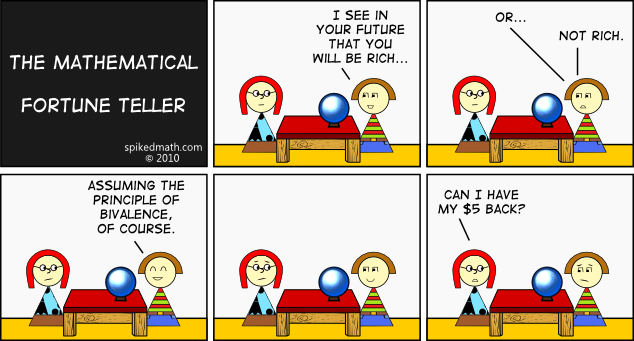
\includegraphics[scale=0.65]{fortune-teller.png}
  \end{center}
}

\frame{\titlepage}
\frame[t]{\scriptsize\tableofcontents}

\section{Einführung}

\subsection{Informale Bedeutung logischer Formeln}
\frame[t]{\frametitle{Informale Bedeutung logischer Formeln}
  \tikz[remember picture] \node[coordinate,yshift=0.7em] (n0) {};
  \vspace{-1.5em}
  \begin{description}\small
    \item[$\bot$] Es stimmt ein Widerspruch.
    \tikz[remember picture] \node[coordinate,yshift=0.0em] (n2) {};
    \item[$A \wedge B$] $A$ und $B$ stimmen.
    \item[$A \vee B$] $A$ oder $B$ stimmt.
    \item[$A \Rightarrow B$] Sollte~$A$ stimmen, dann auch~$B$.
    \item[$\forall x{:}X\_\! A(x)$] Für alle~$x\?X$ stimmt jeweils~$A(x).$
    \item[$\exists x{:}X\_\! A(x)$] Es gibt mindestens ein~$x\?X$, für das~$A(x)$
    stimmt.
    \tikz[remember picture] \node[coordinate,yshift=-0.0em] (n1) {};
  \end{description}
  \vspace{1em}

  \begin{description}\small
    \item[$\bot$] 
    \tikz[remember picture] \node[coordinate,yshift=0.0em] (n5) {};%
    Wir haben Beleg für einen Widerspruch.
    \item[$A \wedge B$] Wir haben Beleg für~$A$ und für~$B$.
    \item[$A \vee B$] Wir haben Beleg für~$A$ oder für~$B$.
    \item[$A \Rightarrow B$] Sollten wir Beleg für~$A$ haben, können wir
    (gleichmäßig) auch Beleg für~$B$ konstruieren.
    \item[$\forall x{:}X\_\! A(x)$] Wir können (gleichmäßig) für alle~$x\?X$
    Belege für~$A(x)$ konstruieren.
    \item[$\exists x{:}X\_\! A(x)$] Wir haben ein~$x\?X$ zusammen mit Beleg
    für~$A(x)$.
    \tikz[remember picture] \node[coordinate,yshift=-0.0em] (n4) {};
  \end{description}

  \begin{tikzpicture}[overlay,remember picture]
    \path (n2) -| node[coordinate] (n3) {} (n0);
    \path (n1) -| node[coordinate] (n33) {} (n0);
    \draw[thick,decorate,decoration={brace,amplitude=5pt}]
            (n33) -- (n3) node[midway,left=4pt] {kl.};
    \path (n5) -| node[coordinate] (n6) {} (n0);
    \path (n4) -| node[coordinate] (n44) {} (n0);
    \draw[thick,decorate,decoration={brace,amplitude=5pt}]
            (n44) -- (n6) node[midway,left=4pt] {int.};
  \end{tikzpicture}

  \begin{tikzpicture}[remember picture,overlay]  
    \node [xshift=-1cm,yshift=-6cm] at (current page.north east)
      {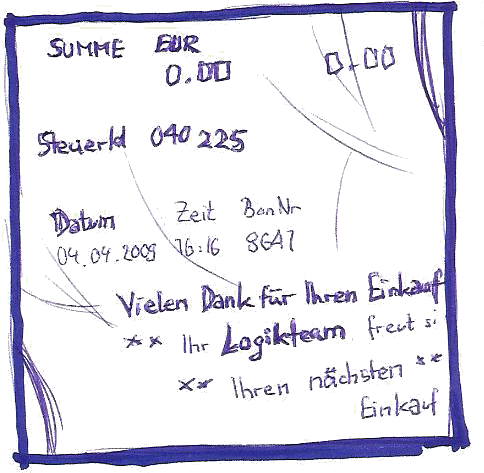
\includegraphics[scale=0.3]{evidence.png}};
  \end{tikzpicture}
}

\subsection{Das Axiom vom ausgeschlossenen Dritten}
\frame[t]{\frametitle{Das Axiom vom ausgeschlossenen Dritten}
  \begin{axiom}[\emph{LEM}, klassisch]
    Für jede Aussage~$A$ kann man
    \[ A \,\vee\, \neg A \]
    ableiten.
  \end{axiom}

  \begin{itemize}
    \item Klassische Interpretation: \\ Eine jede Aussage stimmt oder stimmt nicht.
    \item Intuitionistische Interpretation: \\ Für jede Aussage haben wir jeweils Beleg
    für sie oder für ihre Negation.
    \vfill
    \item intuitionistische Logik $:=$
          klassische Logik ohne LEM
  \end{itemize}

  \begin{tikzpicture}[remember picture,overlay]  
    \node [xshift=-1.7cm,yshift=-3.8cm] at (current page.north east)
      {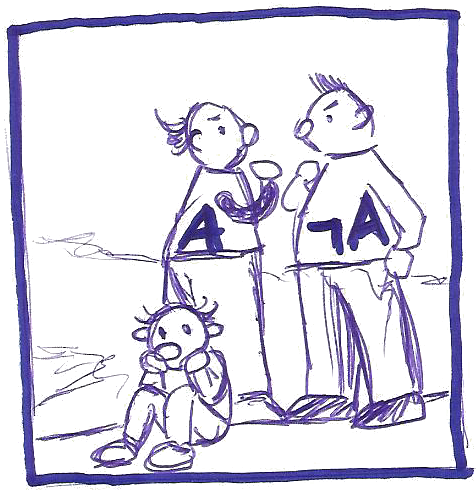
\includegraphics[scale=0.4]{lem.png}};
  \end{tikzpicture}
}

\subsection{Anwendungen}
\frame[t]{\frametitle{Anwendungen}
  \only<1>{
    \begin{center}
      
\includegraphics[scale=0.4]{fun.png}
    \end{center}
  }
  \pause

  \begin{itemize}
    \item Mit intuitionistischer Logik kann man Belegbarkeitsfragen untersuchen.
    \item Aus intuitionistischen Beweisen kann man \emph{Programme} extrahieren.
    \item Die \emph{interne Sprache} von Topoi ist i.\,A. intuitionistisch.
    \item Intuitionistisch kann man \emph{Traummathematik} studieren.
  \end{itemize}

  \vfill
  \begin{center}
    \phantom{a}
    \hfill
    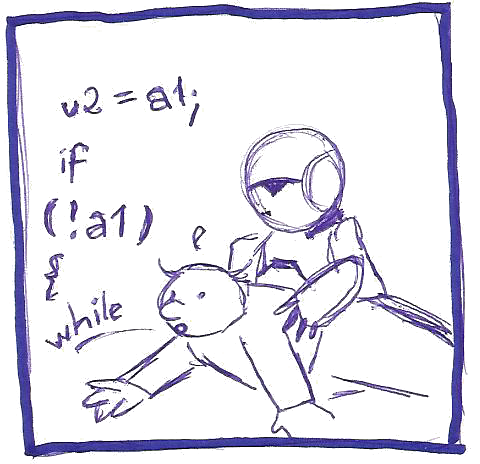
\includegraphics[scale=0.4]{program-extraction.png}
    \hfill
    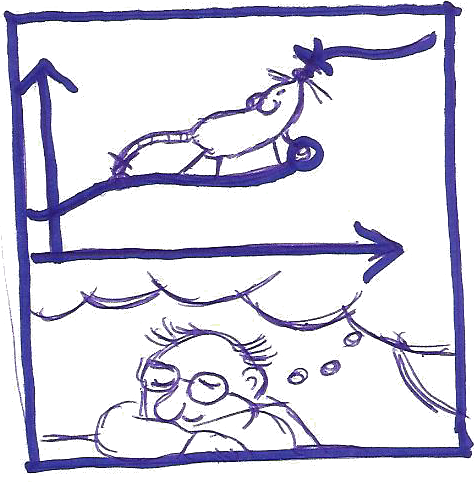
\includegraphics[scale=0.4]{dream-maths.png}
    \hfill
    \phantom{a}
  \end{center}
}

\section{Eine andere mathematische Welt}

% XXX: Fehlt Intro.
% insbes. erklären, dass wir durchaus an not(phi) ^ not(not(phi)) glauben.
\subsection{Leere und nichtleere Mengen}
\frame[t]{\frametitle{Leere und nichtleere Mengen}
  Sei~$X$ eine Menge.
  
  \emph{Frage:} Sind die beiden folgenden Aussagen
  äquivalent?
  \begin{enumerate}
    \item $X$ ist \emph{nicht leer}, d.\,h. $X \neq \emptyset$.
    \item $X$ ist \emph{bewohnt}, d.\,h. $\exists x \in X$.
  \end{enumerate}

  \visible<2>{
  Aussage~{\insertenumlabel} ist stärker: Man kann explizit ein Element~$x$ der
  Menge angeben.
  }

  \vfill
  \begin{center}
    
\includegraphics[scale=0.4]{empty-set.png}
    \hfill
    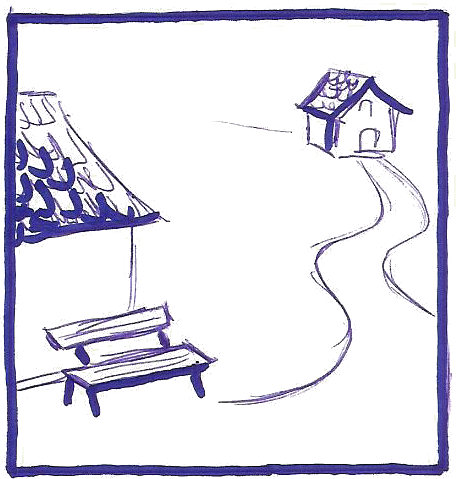
\includegraphics[scale=0.4]{schwebe-set.png}
    \hfill
    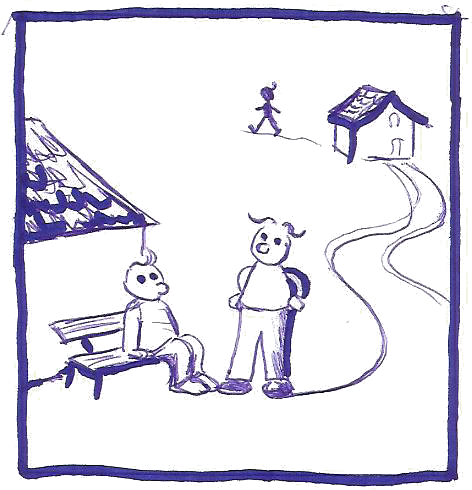
\includegraphics[scale=0.4]{inhabited-set.png}
  \end{center}
}

\subsection{Teilmengen der Eins}
\frame[t]{\frametitle{Teilmengen der Eins}
  \begin{definition}Die \emph{Menge der Wahrheitswerte~$\Omega$} ist
  die Menge aller Teilmengen der Menge
  \[ \1 := \{ \star \}, \]
  also
  \[ \Omega := \P(\1) = \{ U \subseteq \1 \}. \]
  \end{definition}

  \begin{itemize}
    \item \emph{Frage:} Wie viele Elemente enthält~$\Omega$?
    \pause
    \item Es gibt auch
    \begin{align*}
      \Omega_{\text{entscheidbar}} &:= \{ p \in \Omega \,|\, \text{$\star \in p$
      oder $\star \not\in p$} \}, \\
      \Omega_{\text{stabil}} &:= \{ p \in \Omega \,|\, \neg \neg(\star \in
      p) \Rightarrow \star \in p \}.
    \end{align*}
    In welcher Beziehung stehen diese zu~$\Omega$?
  \end{itemize}
}

\subsection{Minima von Mengen natürlicher Zahlen}
\frame[t]{\frametitle{Minima von Mengen natürlicher Zahlen}
  Klassisch gilt: Jede bewohnte Menge natürlicher Zahlen besitzt ein Minimum.

  \emph{Frage:} Stimmt das auch intuitionistisch?

  \vspace{1em}
  \begin{center}
    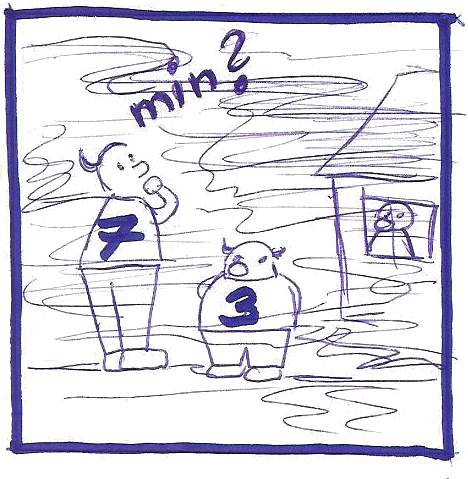
\includegraphics[scale=0.6]{minima.png}
  \end{center}
}

\subsection{Endliche Mengen}
\frame[t]{\frametitle{Endliche Mengen}
  \begin{definition}
    Sei~$X$ eine Menge. $X$ heißt\ldots
    \begin{itemize}
      \item \ldots\emph{endlich} \tabto{3.4cm} $:\Leftrightarrow$
        $\exists n \in \N\_ \exists f{:}\, [n] \to X\_ \text{$f$ bijektiv}$.
      \item \ldots\emph{endlich indiziert} \tabto{3.4cm} $:\Leftrightarrow$
        $\exists n \in \N\_ \exists f{:}\, [n] \to X\_ \text{$f$ surjektiv}$.
    \end{itemize}
    Dabei ist~$[n] := \{ m \in \N \,|\, m < n \} = \{ 0, 1, \ldots, n-1 \}$.
  \end{definition}

  \emph{Frage:} \tabto{1.2cm} Sind Teilmengen endlicher (endl. indizierter) \\
  \tabto{1.2cm} Mengen wieder endlich (endl. indiziert)?

  \begin{tikzpicture}[remember picture,overlay]  
    \node [xshift=-2.0cm,yshift=-7.8cm] at (current page.north east)
      {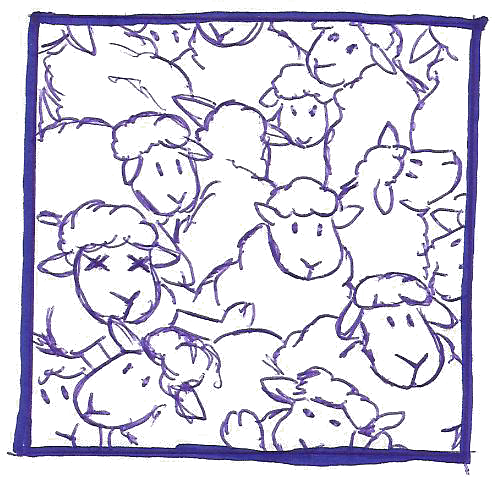
\includegraphics[scale=0.4]{many-sheep.png}};
  \end{tikzpicture}
}


\section{Eleganzassistenz}

\subsection{Unendlichkeit der Primzahlen}
\frame[t]{\frametitle{Unendlichkeit der Primzahlen}
  \begin{theorem}[schwache Form]Die Menge~$\mathbb{P}$ der Primzahlen,
  \[ \mathbb{P} := \{ 2, 3, 5, 7, 11, 13, \ldots \} \subseteq \N, \]
  ist nicht endlich.\end{theorem}
  \pause

  \begin{theorem}[starke Form]Sei~$S$ eine endliche Menge von Primzahlen. Dann gibt es
  eine weitere Primzahl, die nicht in~$S$ enthalten ist.\end{theorem}
}

\subsection{Übungsaufgabe in Linearer Algebra I}
\frame[t]{\frametitle{Übungsaufgabe in Linearer Algebra I}
  \begin{proposition}
    Sei~$f{:}\, X \to Y$ eine Abbildung und sei
    \[ \renewcommand{\arraystretch}{1.3}\begin{array}{@{}rrcl@{}}
      \varphi{:} &\P(Y)&\longrightarrow& \P(X), \\
      & U &\longmapsto& f^{-1}[U] := \{ x \in X \,|\, f(x) \in U \}
    \end{array} \]
    die zugehörige Urbildoperation. Dann ist~$f$ genau dann surjektiv,
    wenn~$\varphi$ injektiv ist.
  \end{proposition}

  \emph{Zum Knobeln:} Auch für die Rückrichtung gibt es einen direkten Beweis.
}


\section{Kalkül natürlichen Schließens}
\frame[t]{\frametitle{Kalkül natürlichen Schließens}
}

\section{Semantik}

\subsection{Heytingalgebren}
\frame[t]{\frametitle{Heytingalgebren}
  \begin{definition}
    Eine \emph{Heytingalgebra}~$H$ ist eine partiell geordnete Menge~($\leq$), in der
    \begin{enumerate}
    \item alle endlichen Infima~($\sqcap$) und Suprema~($\sqcup$) existieren,
    \item zu je zwei Elementen~$a,b \in H$ ein Element $(a \to b) \in H$ mit
    \[ x \sqcap a \leq b \quad\text{gdw.}\quad x \leq (a \to b) \]
    für alle~$x \in H$ existiert.
    \end{enumerate}
  \end{definition}

  \vfill
  \begin{itemize}
    \item Beispiele für Heytingalgebren: $\{ 0, \nicefrac{1}{2}, 1\}$, $\P(\1)$, $\O(X)$
    \item Nutzen als Modelle für intuitionistische propositionale Logik
  \end{itemize}
}

\subsection{Kripkemodelle}
\frame[t]{\frametitle{Kripkemodelle}
  \begin{definition}
    Ein \emph{Kripkemodell} besteht aus
    \begin{enumerate}
      \item einer partiell geordneten Menge~$W$ von Welten und
      \item einer Erfüllbarkeitsrelation~$\models$
    \end{enumerate}
    sodass folgende Axiome erfüllt sind:
    \begin{enumerate}
      \item Aus $w \leq u$ und $w \models A$ folgt $u \models A$.
      \item $w \models \bot$ stimmt nicht.
      \item $w \models A \wedge B$ \tabto{2.3cm} gdw. $w \models A$ und $w \models B$.
      \item $w \models A \vee B$ \tabto{2.3cm} gdw. $w \models A$ oder $w \models B$.
      \item $w \models A \Rightarrow B$ \tabto{2.3cm} gdw. für alle~$u$ mit~$w
      \leq u$: \\ \tabto{2.3cm} ${\qquad}$ Aus $u \models A$ folgt $u \models B$.
    \end{enumerate}
  \end{definition}
}

\section{Doppelnegationsübersetzung}
\frame[t]{\frametitle{Doppelnegationsübersetzung}
  \begin{definition}
    \begin{itemize}
      \item
        Eine Aussage~$A$ heißt genau dann \emph{entscheidbar}, wenn
        \[ A \ \vee\  \neg A. \]
      \item
        Eine Aussage~$A$ heißt genau dann \emph{stabil}, wenn
        \[ \neg\neg A \ \Rightarrow\  A. \]
    \end{itemize}
  \end{definition}

  \vfill
  Beispiele:
  \begin{itemize}
    \item "`$n = m$"' ist für natürliche Zahlen $n$, $m$ entscheidbar.
    \item Entscheidbare Aussagen sind auch stabil.
    \item Jede Aussage der Form $\neg\neg B$ ist stabil.
  \end{itemize}
}

% Äquikonsistenzresultat

\end{document}
